%% Expensitor -- IEEE conference paper SKELETON
%%
%% Compile with pdflatex + bibtex (or drop the folder into Overleaf).
%% This is a scaffold with your REAL measured seed-set numbers wired in and
%% every "you still need this" gap marked \todo{...}. Do not submit as-is:
%% fill the placeholders, run the harness on real datasets, add the user study,
%% and VERIFY every citation in DBLP/IEEE Xplore (see paper/README.md).

\documentclass[conference]{IEEEtran}
\IEEEoverridecommandlockouts

\usepackage{cite}
\usepackage{amsmath,amssymb,amsfonts}
\usepackage{algorithmic}
\usepackage{graphicx}
\graphicspath{{figures/}}
\usepackage{textcomp}
\usepackage{xcolor}
\usepackage{booktabs}
\usepackage{url}

% Placeholder highlighter -- remove \usepackage + redefine to no-op before submit.
\newcommand{\todo}[1]{{\color{red}\textbf{[TODO: #1]}}}

\def\BibTeX{{\rm B\kern-.05em{\sc i\kern-.025em b}\kern-.08em
    T\kern-.1667em\lower.7ex\hbox{E}\kern-.125emX}}

\begin{document}

\title{Expensitor: A Privacy-Preserving, On-Device, Deterministic\\
Personal-Finance Companion}

\author{
\IEEEauthorblockN{\todo{Author Name(s)}}
\IEEEauthorblockA{\todo{Department, Institution}\\
\todo{City, Country}\\
\todo{email@domain}}
}

\maketitle

\begin{abstract}
Modern personal-finance assistants increasingly rely on cloud services, large
language models (LLMs), and pooled user data to capture and categorise spending.
This raises three coupled concerns: user privacy (financial data leaving the
device), recurring cost and latency (per-request cloud/LLM calls), and
explainability (opaque model decisions over money). We present \emph{Expensitor},
a personal-finance companion built on the opposite set of choices: capture and
reasoning are \emph{deterministic}, run \emph{on-device} or from the user's own
data, and function \emph{offline}, with an optional \emph{local} model used only
for conversational phrasing and never as a source of numeric fact. The system
captures transactions from bank SMS alerts and photographed receipts using
rule-based extraction with on-device OCR, and introduces an amount-aware
adaptive reason-suggestion method that ranks a user's own past spend reasons so
that recording a recurring expense is a single tap. We evaluate the components
with a reproducible harness. On hand-labelled seed sets, transaction detection
reaches an F\textsubscript{1} of 0.931 with perfect precision (zero false
positives across ten non-transaction message classes), receipt line-item
extraction reaches F\textsubscript{1} 0.971, and the amount-aware reason ranking
achieves Hit@1 of 0.667, roughly three times a frequency/recency baseline.
We frame the contribution as a \emph{system and evaluation}: not a new extraction
model, but a quantified demonstration that a privacy-preserving, explainable,
on-device design is a viable point in the design space.
\todo{Add one sentence with the real-dataset + user-study headline once collected.}
\end{abstract}

\begin{IEEEkeywords}
personal finance, on-device computing, privacy, deterministic systems, receipt
OCR, SMS parsing, expense tracking, human-computer interaction
\end{IEEEkeywords}

\section{Introduction}
Personal financial management (PFM) applications are a mature and crowded space,
and recent systems increasingly delegate transaction understanding to cloud
pipelines and LLMs. That trend improves convenience but concentrates sensitive
data off-device and makes each interaction dependent on network access, cloud
cost, and non-deterministic model behaviour.

This paper asks whether a genuinely useful PFM companion can be built while
holding the opposite line: \emph{no cloud OCR, no third-party transaction API,
no pooled cross-user model, and no paid LLM}. Our thesis is that the resulting
privacy, offline capability, and explainability are worth a measured accuracy
trade-off, and that this trade-off can be quantified rather than merely claimed.

\textbf{Contributions.}
\begin{itemize}
\item A PFM companion whose capture and reasoning are deterministic, on-device
      or user-data-local, and offline-capable, with an optional \emph{local}
      model behind a rules fallback (Sec.~\ref{sec:system}).
\item An amount-aware adaptive reason-suggestion method that ranks a user's own
      past reasons for one-tap recording (Sec.~\ref{sec:reasons}).
\item A reproducible evaluation harness and results quantifying the accuracy of
      each component against baselines (Sec.~\ref{sec:eval}), released with the
      system.
\end{itemize}

\section{Related Work}
\label{sec:related}
% VERIFY every citation below before submission (paper/README.md). Do not cite a
% paper you have not read.
\textbf{SMS-based transaction extraction.} Extracting transactions from bank SMS
alerts is well studied, particularly in the Indian context where regulators
mandate per-transaction alerts, and both rule-based and learned approaches
exist~\cite{smssmsref, nlpframework}. Public datasets support benchmarking
this task~\cite{kagglesms}.

\textbf{Receipt understanding.} Scanned-receipt OCR and information extraction is
a mature area, standardised by the ICDAR-2019 SROIE
competition~\cite{sroie} and advanced by transformer and multimodal
models~\cite{receiptmm}; commercial systems report line-item accuracy above
99\%~\cite{veryfi}.

\textbf{ML for spending analysis.} A large body of work applies machine learning
to expense categorisation, forecasting, and behaviour
analysis~\cite{pfmml, smartexpense}.

\textbf{Positioning.} These works optimise extraction accuracy, typically with
cloud or learned models. Our contribution is orthogonal: we hold accuracy as a
\emph{constraint} while optimising for privacy, determinism, offline operation,
and explainability, and we quantify the resulting system. To our knowledge this
specific combination, evaluated as a whole, is not covered by the above.
\todo{After verifying citations, add 2--3 sentences contrasting Expensitor with
the single closest prior system by name.}

\section{System Design}
\label{sec:system}
Expensitor comprises a Flutter mobile client and a FastAPI backend with an
asynchronous PostgreSQL store (Fig.~\ref{fig:arch}). Financial reasoning
(projection, feasibility, behavioural profiling, savings) is implemented as
deterministic Python modules that compute results from stored facts on read;
there is no background scheduler and no learned model in the numeric path.

\begin{figure}[t]
\centering
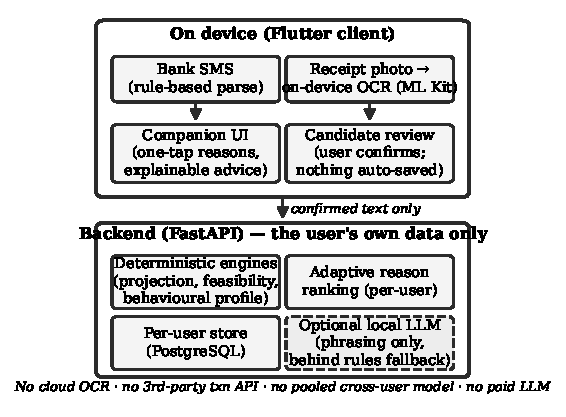
\includegraphics[width=\columnwidth]{fig_architecture.pdf}
\caption{System architecture and privacy boundary. Bank-SMS parsing and receipt
OCR run on-device; the deterministic reasoning engines operate on the user's own
data. No cloud OCR, third-party transaction API, or pooled cross-user model is
used, and the optional local LLM only phrases output, behind a rules fallback.}
\label{fig:arch}
\end{figure}

\textbf{Privacy properties.} (i) Receipt OCR runs on-device (Google ML Kit),
so images never leave the phone; only text the user confirms is stored.
(ii) Transactions are captured from the user's own bank SMS, not a third-party
account-aggregation API. (iii) Learned artefacts (reasons, item prices,
behavioural patterns) are strictly per-user and never pooled into a shared
model. (iv) An optional \emph{local} LLM (Ollama) is used only for
natural-language phrasing and free-text intent, always behind a deterministic
fallback, and never as a source of a numeric value.

\textbf{Capture.} Bank SMS messages are parsed by a rule-based extractor that
first \emph{rejects} non-transactions (one-time passwords, promotions, balance
notifications, payment requests, failures, scheduled debits) before extracting
amount, direction, and merchant. Receipts are parsed from on-device OCR text
into a merchant, total, and line items, preferring an explicitly labelled total
over subtotal/tax lines. Both produce \emph{candidates} that the user confirms;
nothing is recorded automatically, bounding the cost of a misread.

\section{Adaptive Reason Suggestion}
\label{sec:reasons}
When recording a spend, the system ranks the user's own past reasons so the
correct one is typically a single tap. For each distinct past reason $r$ we
compute a score for a target amount $a$ on date $d$:
\begin{equation}
\mathrm{score}(r) = \underbrace{\sqrt{w(r)}}_{\text{base}} \cdot
\underbrace{\big(1 + \beta_1 \phi_{\mathrm{wd}} + \beta_2 \phi_{\mathrm{cat}}\big)}_{\text{context boost}} \cdot
\underbrace{g(r, a)}_{\text{amount gate}}
\end{equation}
where $w(r) = \sum_{t \in T_r} 2^{-\Delta(t,d)/h}$ is a recency-weighted use
count over the reason's past occurrences $T_r$ (half-life $h$), so that stale
reasons decay; $\phi_{\mathrm{wd}}, \phi_{\mathrm{cat}} \in [0,1]$ are the
fractions of $r$'s uses matching the target weekday and category; and the
amount gate
\begin{equation}
g(r,a) = \gamma + (1-\gamma)\, e^{-2\,|{m_r - a}|/a}
\end{equation}
multiplies the score toward a floor $\gamma$ when $r$'s median amount $m_r$ is
far from $a$. The gate is the key design choice: a reason whose usual amount is
far from the current spend cannot win on frequency alone (e.g. a frequent
low-value ``chai'' reason does not surface for a large grocery spend). When no
amount is supplied the gate is neutral. All quantities derive only from the
user's own history.

\section{Evaluation}
\label{sec:eval}
We evaluate the three measurable components with a seeded, offline harness
released with the system. Unless stated, results are on hand-labelled seed
datasets and therefore represent clean-input performance; Sec.~\ref{sec:limits}
discusses this.

\subsection{Bank-SMS transaction extraction}
On a labelled set of \todo{N} messages (\todo{$P$} transactions, \todo{$Q$}
non-transactions across ten message classes), we measure detection
(transaction vs.\ not) against a naive ``any currency amount is a transaction''
baseline, and field extraction on correctly-detected transactions.
Table~\ref{tab:sms} reports the seed-set result.

% Table generated by paper/build_assets.py from the harness output.
% GENERATED by paper/build_assets.py from research/generated/results.json (do not edit).
\begin{table}[t]
\caption{Bank-SMS detection (seed set, 51 messages: 31 transactions, 20 non-transactions).}
\label{tab:sms}
\centering
\begin{tabular}{lcccc}
\toprule
Method & Precision & Recall & F\textsubscript{1} & Accuracy\\
\midrule
Expensitor (rules) & \textbf{1.000} & 0.871 & \textbf{0.931} & \textbf{0.922}\\
Baseline (any amount) & 0.660 & \textbf{1.000} & 0.795 & 0.686\\
\bottomrule
\end{tabular}
\end{table}


Field extraction on the detected transactions: direction accuracy 1.000, amount
exact-match 1.000, merchant exact-match 0.926. Critically, the parser produced
\emph{zero} false positives across all non-transaction classes (OTP, promotion,
balance, request, failure, reminder, scheduled, refund, notice, unrelated). The
result characterises a deliberate operating point: near-perfect precision at the
cost of recall (missed transaction formats), appropriate when the alternative to
a missed capture is a one-tap manual entry, whereas a false capture is a
corrupted ledger. \todo{Re-run on the Kaggle Indian-bank-SMS corpus and report;
expect lower recall under format diversity.}

\subsection{Receipt extraction}
On \todo{N} labelled samples, we measure receipt detection, total and merchant
exact-match, and line-item extraction as precision/recall/F\textsubscript{1}
over (name, price) pairs (Table~\ref{tab:receipt}).

% Table generated by paper/build_assets.py from the harness output.
% GENERATED by paper/build_assets.py from research/generated/results.json (do not edit).
\begin{table}[t]
\caption{Receipt extraction (seed set, 15 samples, clean text).}
\label{tab:receipt}
\centering
\begin{tabular}{lc}
\toprule
Metric & Score\\
\midrule
Receipt detection F\textsubscript{1} & 1.000\\
Total exact-match & 1.000\\
Merchant exact-match & 1.000\\
Line-item F\textsubscript{1} (P 0.944 / R 1.000) & 0.971\\
\bottomrule
\end{tabular}
\end{table}


These numbers are on clean labelled text and therefore upper-bound real
performance. \todo{Re-run on ICDAR-2019 SROIE to report under genuine OCR noise;
this is required for the claim to be credible.}

\subsection{Adaptive reason suggestion}
We evaluate the ranking on a seeded 90-day synthetic history with latent
patterns (e.g.\ a low-value daily reason, a weekly high-value reason) plus noise.
Held-out probes (a typical amount with an unambiguous true reason, absent from
the history) test whether the true reason is surfaced. We report Hit@1, Hit@3,
and mean reciprocal rank against most-frequent, most-recent, and random
baselines (Table~\ref{tab:reasons}).

% Table generated by paper/build_assets.py from the harness output.
% GENERATED by paper/build_assets.py from research/generated/results.json (do not edit).
\begin{table}[t]
\caption{Reason-suggestion ranking (9 synthetic held-out probes over a 90-day history).}
\label{tab:reasons}
\centering
\begin{tabular}{lccc}
\toprule
Method & Hit@1 & Hit@3 & MRR\\
\midrule
Expensitor (amount-aware) & \textbf{0.667} & \textbf{0.778} & \textbf{0.731}\\
Most-frequent & 0.222 & 0.444 & 0.414\\
Most-recent & 0.222 & 0.444 & 0.407\\
Random & 0.222 & 0.222 & 0.345\\
\bottomrule
\end{tabular}
\end{table}


\begin{figure}[t]
\centering
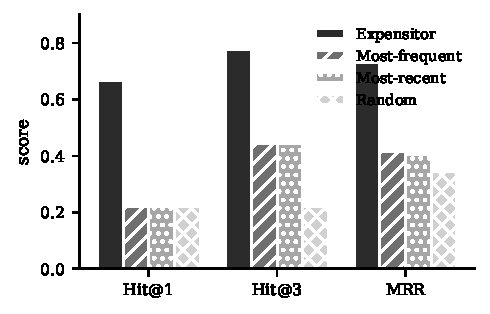
\includegraphics[width=\columnwidth]{fig_reason_ranking.pdf}
\caption{Amount-aware reason ranking vs.\ frequency, recency, and random
baselines on the held-out probes. The amount gate roughly triples Hit@1.}
\label{fig:reasons}
\end{figure}

The amount-aware ranking roughly triples Hit@1 over the baselines
(Fig.~\ref{fig:reasons}), confirming that the amount gate carries most of the
signal. \todo{Replace or supplement with a real logged-usage evaluation once
available.}

\subsection{Optional: deterministic vs.\ LLM baseline}
\todo{Run the SMS/receipt tasks through the local LLM via the same harness and
report accuracy, latency, and on-device feasibility, to quantify the trade the
paper argues for.}

\subsection{User study}
\todo{Report a study (target $N=15$--$30$): System Usability Scale, and
task-completion time for recording a spend (tap-a-suggested-reason vs.\ manual
entry). Obtain institutional consent/ethics approval before running.}

\section{Limitations and Threats to Validity}
\label{sec:limits}
\textbf{Dataset scale and cleanliness.} The seed sets are small and hand-labelled
on clean text; the SMS and receipt numbers upper-bound field performance and
must be re-established on the Kaggle corpus and SROIE respectively.
\textbf{Synthetic ranking evaluation.} The reason-ranking result demonstrates the
mechanism without leakage but is not a real-usage study.
\textbf{Rule-based ceiling.} The extractors are deliberately rule-based; the
contribution is the system and its privacy/determinism properties, not
state-of-the-art extraction accuracy.
\textbf{Generality.} Rules are tuned to Indian bank-SMS conventions and English
receipts; other locales require extension.

\section{Conclusion and Future Work}
We presented Expensitor, a personal-finance companion that deliberately trades a
measured amount of extraction accuracy for privacy, determinism, offline
operation, and explainability, and quantified each component with a reproducible
harness. Future work includes the real-dataset and user-study evaluations noted
above, an anonymised regional price-comparison layer with formal privacy
guarantees, and extension to further locales.

\section*{Reproducibility}
The system, the evaluation harness, and the seed datasets are available at
\todo{repository URL}. Every number, table, and result figure in this paper is
generated from the code over the checked-in data: the harness
(\texttt{make\_results}) writes a JSON of all metrics, and a build script turns
that JSON into the \LaTeX{} tables and figures here---none are hand-transcribed.
The evaluation is deterministic (seed sets and a fixed random seed), so a
re-run reproduces the JSON byte-for-byte.

\begin{thebibliography}{00}
\bibitem{smssmsref} \todo{VERIFY} Rule-based transaction extraction from bank SMS
alerts, IEEE Int. Conf. (surfaced in search; confirm authors/venue/year in DBLP
before citing).
\bibitem{nlpframework} \todo{VERIFY} NLP framework for automated expense
management from transactional messages (confirm venue/year).
\bibitem{kagglesms} Indian Banking Transaction Text Dataset, Kaggle.
\url{https://www.kaggle.com/datasets/coderanand/indian-banking-transaction-text-dataset}
\bibitem{sroie} ICDAR2019 Competition on Scanned Receipt OCR and Information
Extraction (SROIE). \url{https://arxiv.org/abs/2103.10213}
\bibitem{receiptmm} \todo{VERIFY} Receipt information extraction with multimodal
transformer and rule-based methods (confirm exact reference).
\bibitem{veryfi} Line-item extraction accuracy benchmarks (industry report).
\url{https://www.veryfi.com/technology/line-item-extraction-accuracy-benchmarks/}
\bibitem{pfmml} \todo{VERIFY} Personal Finance Management and Prediction using ML,
IEEE. \url{https://ieeexplore.ieee.org/document/10816949/}
\bibitem{smartexpense} \todo{VERIFY} Smart Expense Tracking System Using Machine
Learning (confirm venue/year).
\end{thebibliography}

\end{document}
